\documentclass[11pt]{article}
\setlength\parindent{0pt}
\usepackage{amsmath}
\usepackage{amsfonts}
\usepackage{graphicx}
\newcommand{\reffig}[1]{[Figure \ref{#1}]}
\title{Independent Study Project}
\author{Zachary Kieda\\{Advisor: Jesse Stiles}}
\date{\today}
\begin{document}
\maketitle

Our project has three major components -- music generation, music visualization in two dimensions, and music visualization in three dimensions using the Oculus Rift. The music generation uses a modified version basic machine learning technique, $n$-grams. The music generation software, along with the music visualization software in two dimensions was written from the ground-up in Java. The three dimensional visualization is written in Unity to set up and create the scene, while the camera controller and the controller for the visualization is in C\#. We wrote the shaders for our 3d visualization in HLSL so we could use the GPU to improve performance.\\

The Java project with the two dimensional visualization is written completely in Java, and directly controls the parameters for the visualization. When we are using the oculus, the Java side still produces and plays music, but passes the visualization parameters to the C\# side.\\

The 2d visualization is an interesting pattern based on modular arithmetic that is meant to oscillate according to the music being played. The 3d visualization wraps this over a sphere, and applies a generated albedo map and height map that causes the surface to bump out. The user views the visualization move in realtime using the oculus rift, and can navigate and look around the inside of the sphere.\\

We have encountered several problems while working on this project, and have had to make appropriate modifications in order for the project to work. Most notably, C\# lacks a sufficiently complex midi encoder/ decoder or midi player library that I could find online. As well, I already wrote the music generation and midi processing in Java. It's important to note that C\# and Java do not particularly interface well. In order for our project to work, we had to write a client/server interaction on the C\# and Java sides so the two could communicate locally. The Java component has the responsibility of generating midi, producing sound, and computing how the visualization should change over time. The C\# component takes information about the current state of the visualization, translates that and changes the parameters of our visualization accordingly. The C\# component then displays the visualization on a sphere which we can navigate in three dimensional space. \\

Another problem is with the Java midi player itself. In order to play the midi sound to a three dimensional environment, we would have to get a \verb|AudioInputStream| and play it through java 3d sounds. This means that when a midi sound is played we would have to get its underlying \verb|AudioOutputStream| and pass it to a \verb|PipedOutputStream| for us to modify the sound being produced before sending it to the speakers. However, after searching through the Java SDK, we found that the \verb|AudioOutputStream| produced is inaccessible, and the only way to get it is to copy a large portion of the java midi SDK, modifying particular portions in order to get this sound. So, we settled for the music produced to be in mono. A final option would be to send the midi to MaxMSP through a port and let MaxMSP control the three dimensional position using the ambisonics library. Due to time constraints this has not been implemented, but we find that our project does fine without it. \\

We experimentally found interesting points and mappings to control the visualization. In order to do this conveniently and efficiently, we created the `Ground Control' program that allows us to easily change the parameters of our visualizations and adjust it to the music generated. You can start the program with ground control by setting \verb|useController = true| in \verb|edu.cmu.ideate.zkieda.viz.drivers.Main|. The ground control is shown below.\\
\begin{center}
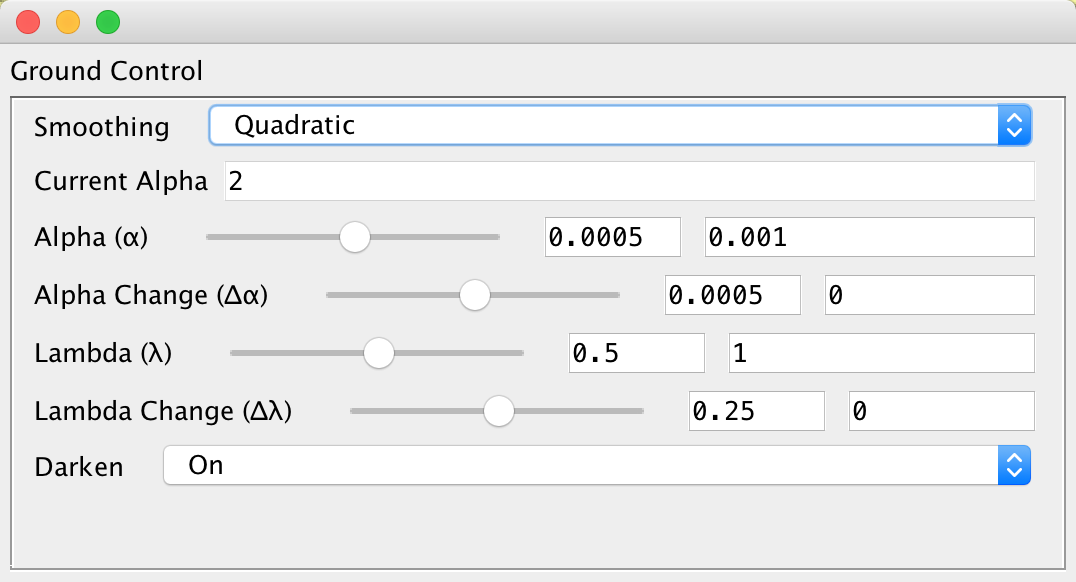
\includegraphics[width=\textwidth]{ground-control.png}\\
Figure 1: Major Tom, the Ground Control
\end{center}
\end{document}